\documentclass[11pt]{article}  
\usepackage[margin=1in]{geometry}
\usepackage{authblk}
\usepackage{graphicx}
\usepackage{amsmath}

\usepackage{ltexpprt} 

\title{Multi-Commodity Flow with In-Network Processing}
\author{Moses Charikar, Yonatan Naamad, Jennifer Rexford, and X. Kelvin Zou\\
Department of Computer Science, Princeton University\\
\texttt{\{moses,ynaamad,jrex,xuanz\}@cs.princeton.edu}}
\date{}

\begin{document}
\maketitle
\thispagestyle{empty}

\section{Introduction}
%%%
%%% Middleboxes are important
%%%
In addition to delivering data efficiently, today's computer networks often perform services on the traffic in flight to enhance security, privacy, or performance, or provide new features.  Network administrators frequently install so-called ``middleboxes'' such as firewalls, network address translators, server load balancers, Web caches, video transcoders, and devices that compress or encrypt the traffic.  In fact, many networks have as many middleboxes as they do underlying routers or switches.  Often a single conversation, or \emph{connection}, must traverse multiple middleboxes, and different connections may go through different sequences of middleboxes.  For example, while Web traffic may go through a firewall followed by a server load balancer, video traffic may simply go through a transcoder.  In some cases, the traffic volume is so high that an organization needs to run multiple instances of the same middlebox to keep up with the demand.  Deciding how many middleboxes to run, where to place them, and how to direct traffic through them is a major challenge facing network administrators.

%%%
%%% Dedicated appliances stink
%%%
Until recently, each middlebox was a dedicated appliance, consisting of both software and hardware.  Administrators tended to install these appliances at critical locations that naturally see most of the traffic, such as the gateway connecting a campus or company to the rest of the Internet.  A network could easily have a long chain of these appliances at one location, forcing all connections to traverse every appliance---whether they need all of the services or not.  In addition, placing middleboxes only at the gateway does not serve the organization's many \emph{internal} connections, unless the internal traffic is routed circuitously through the gateway.
%
%%%
%%% Network Function Virtualization
%%%
Over the last few years, middleboxes are increasingly \emph{virtualized}, with the software service separate from the physical hardware.  Middleboxes now run as virtual machines that can easily spin up (or down) on any physical server, as needed.  This has led to a growing interest in good algorithms that optimize the (i) \emph{placement} of middleboxes over a pool of server resources, (ii) \emph{steering} of traffic through a suitable sequence of middleboxes based on a high-level policy, and (iii) \emph{routing} of the traffic between the servers over efficient network paths~\cite{SIMPLE2013}.

%%%
%%% Combining the optimization problems
%%%
Rather than solving these three optimization problems separately, we introduce---and solve---a joint optimization problem.  Since server resources are fungible, we argue that each compute node could subdivide its resources arbitrarily across any of the middlebox functions, as needed.  That is, the \emph{placement} problem is more naturally a question of what fraction of each node's computational (or memory) resources to allocate to each middlebox function.  Similarly, each connection can have its middlebox processing performed on any node, or set of nodes, that have sufficient resources.  That is, the \emph{steering} problem is more naturally a question of how to decide which nodes should devote a share of its processing resources to a particular portion of the traffic.  Hence, the joint optimization problem ultimately devolves to a new kind of \emph{routing} problem, where we must compute paths through the network based on both the bandwidth and processing requirements of the traffic between each source-sink pair.  That is, a flow from source to sink must be allocated (i) a certain amount of bandwidth on every link in its path and (ii) a total amount of computation across all of the nodes in its path.

\subsection{The Problem}
We can abstract the flow in-network process problem in the following way: there is a flow demand with multi-sources and multi-sinks, and each flow requires a certain amount of in-network (MBox) processing. The in-network processing required for a flow is proportional to the flow size and without losing generality, we assume one unit of flow requires one unit of processing. For a flow from a source to a sink, we assume it is an aggregate flow so the routing and in-network processing for a flow are both divisible. In this model there are two types of constraints: edge capacity and vertex capacity, which represents bandwidth and MBox processing capacity. A feasible flow pattern satisfies: the sum of flows on each edge is bounded by the edge capacity, the sum of in-network process done at each vertex is bounded by the vertex capacity, and the processing done at all vertices for a flow should be equal to flow size and the processing has to be carried out by the flow.

Network design problems involve finding a network with a minimum cost that satisfies various properties, often related to routing and flow feasibility. The network design problem in this model is: for a multi-source and multi-sink flow demand, and a fixed amount of budget to install the processing capacities in the vertices, what is the optimal way to allocate them such that the flow pattern satisfies all the constraints.

Our model is a superset of multi-commodity flow model\cite{MCF}, that is, if we can solve this problem, we can naturally solve multi-commodity flow problem: simply assign each vertex with an infinite capacity it becomes an MCF problem. Many classic MCF design properties can be extended to this problem, such as MC-BB(multi-commodity buy-at-bulk) problem\cite{BuyAtBulk,Charikar05,Chekuri2007}. 
%This paper takes the second approach and show that the decision can be answered via generalized linear programming model for a fractional solution, and have a logarithm approximation for a more practical integer placement.

\begin{figure}[h]
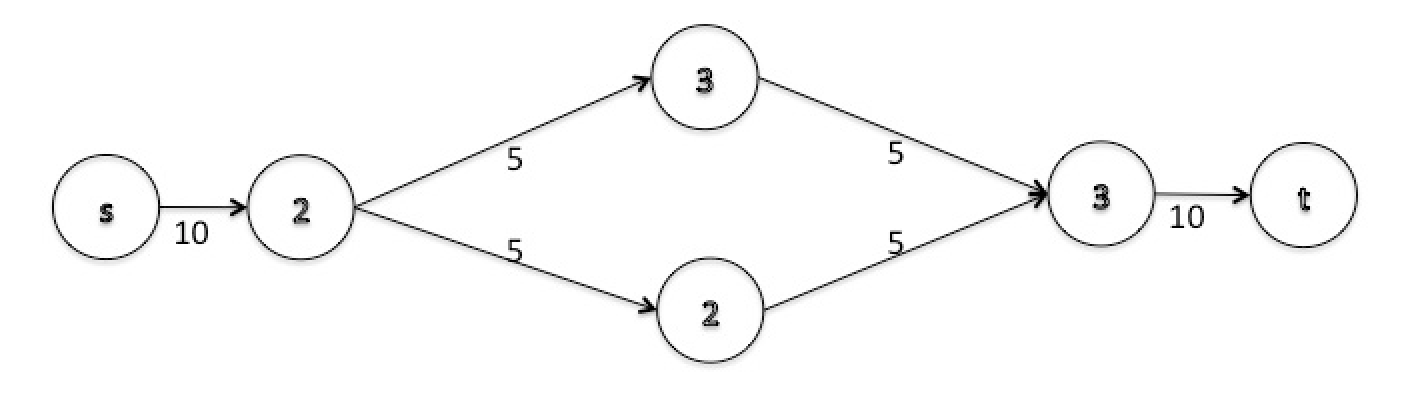
\includegraphics[width=\linewidth]{picture1.png} 
\caption{ \textbf{Example for the Graph Model: given the edge and vertex constraints, \textnormal{\{5,10\} }are edge capacities and \{2,3\} are vertex capacities, the maximum flow from source to sink in the example is 10, in this example all edges and vertices will be saturated.} }
 \end{figure}
\subsection{Notations}
To capture both the capacitated vertices and edges, we use the following notations:
a directed graph $G(V,E)$ where each edge $e\in E$ has an edge bandwidth $B(e)$, and each vertex $v\in V$ has a processing capacity $C(v)$. 

 


\subsection{The results in this paper}



\section{Processing Capacity Placement in fractional manner}
We formulate a generalized linear programming model in this problem in an edge based formulation. Notations: $C(v),B(e)$ represents the processing and edge capacity at node $v$ and edge $e$, $f_i(e)$ represents the flow size for each source-sink pair on edge $e$, $w_i(e)$ represents process demand for flow i carried out at edge $e$, $f(C(v))$ is an concave cost function of $C(v)$: 

\begin{subequations}
\begin{align}
\text{Minimize:}&\sum\limits_v f(C(v))\\
\text{Subject to:}&\forall v \in V-\{s, t\}, \forall i, \sum\limits_{in}  f_i(e)=  \sum\limits_{out} f_i(e);\\
&\forall e, \sum\limits_{i} f_{i}(e)\leq B(e);\\
&\forall e,\forall  i,0 \leq w_i(e) \leq f_i(e),\\
&\forall v,\forall  i, 0\leq \sum\limits_{in } w_i(e) - \sum\limits_{out} w_i(e)   \leq{C(v)}.\\
%&\forall i, \sum\limits_v f_i(s, v) = r_i; \\
&\forall  i; \forall (s, v), w_i = f_i\;\&\; \forall (v,t), w_i =0.
\end{align}
\end{subequations}




\bibliographystyle{acm}
\bibliography{references}

\appendix
\end{document}